\chapter{Introduction}
\label{chap:intro}

% TODO: updates to make:
% - 1.1 MIMO Channel overview
% 	- Add more discussion about MIMO CSI, capacity, precoding/beamforming, 
%	- Add details about 3GPP specificaions (possibly from latest preprint?)
% - Add more 

% Section \ref{sect:notation} introduces the notation used through this work.
This dissertation details work in improving the accuracy and efficiency of deep learning methods for MIMO channel state information estimation. This chapter provides the necessary background to understand the contributions of the dissertation. Section \ref{sect:mimo_model} provides an overview of the MIMO channel and the importance of CSI estimation in MIMO-based communications networks. Section \ref{sect:channel_model} discusses MIMO channel models and introduces the primary channel model used in this work, the COST2100 model. Section \ref{sect:classic_estimation} discusses prior work in compressed sensing for CSI estimation. Section \ref{sect:dl_overview} provides a generic overview of deep learning. 
Boldface lowercase (uppercase) letters indicate vectors (matrices). Unless otherwise specified, the norm $\|\cdot\|$ indicates the Frobenius norm. Superscripts $^T$ ($^H$) indicate the transpose (Hermitian transpose).
% recent work in deep learning for CSI estimation in MIMO networks

\section{MIMO Channel Overview}
\label{sect:mimo_model}

\begin{figure}[!hbtp]
\centering
{
	\fontsize{6pt}{8pt}
	\def\svgwidth{0.8\columnwidth}
	\input{images/mimo-schematic.pdf_tex}
}
\caption{Example multi-antenna transmitter (BS, gNB) and single-antenna user equipment (UE) and relevant system values.}
\label{fig:mimo_schematic}
\end{figure}

In this work, we consider a MIMO channel with a multiple antennas ($N_B \gg 1$) at the transmitter (gNodeB or gNB) servicing a single user equipment (UE) with a single antenna. Under orthogonal frequency division multiplexing (OFDM) with $N_f$ subcarriers, the received symbols on the $m$-th subcarrier for the downlink and the uplink at the receiver are given as
\begin{align*}
	y_{d,m} &= \mathbf h_{d,m}^H\mathbf w_{t,m}x_{d,m} + n_{d,m}.
	% y_{u,m} &= \mathbf w_{r,m}^H\mathbf h_{u,m}x_{u,m} + \mathbf w_{r,m}^H\mathbf n_{u,m},
\end{align*}
where the individual system values are defined in Table~\ref{tab:mimo-params}, and a representative system model is viewable in Figure~\ref{fig:mimo_schematic}. The resulting downlink and uplink channel state information (CSI) matrices are given as
\begin{align*} 
	\bar{\mathbf H}_d &= \begin{bmatrix} \mathbf h_{d,1} & \dots & \mathbf h_{d,N_f}\end{bmatrix}^H \in \mathbb C^{N_f \times N_b}.
	% \bar{\mathbf H}_u &= \begin{bmatrix} \mathbf h_{u,1} & \dots & \mathbf h_{u,N_f}\end{bmatrix}^H \in \mathbb C^{N_f \times N_b}.
\end{align*}
\begin{table}[]
\renewcommand{\arraystretch}{1.25}
\centering
\caption{MIMO system variables considered in this work.}
\label{tab:mimo-params}
\begin{tabular}{c|c|l}
\toprule
\textbf{Symbol}   	  	  & \textbf{Dimension}            & \textbf{Description} \\ \midrule
$y_{d,m}$ 		  	  	  & $\mathbb{C}^{1}$ 			  & Received downlink symbol on $m$-th subcarrier  \\ \hline
$\mathbf h_{d,m}$ 	  	  & $\mathbb{C}^{N_b \times 1}$   & Downlink channel on $m$-th subcarrier  \\ \hline
$\bar{\mathbf H}_{d}$ 	  & $\mathbb{C}^{N_f \times N_b}$ & Downlink CSI (spatial-frequency domain)  \\ \hline
$\mathbf w_{t,m}$ 	  	  & $\mathbb{C}^{N_b \times 1}$   & Transmitter precoding vector for $m$-th subcarrier  \\ \hline
$x_{d,m}$ 		  	  	  & $\mathbb{C}^{1}$ 			  & Trasmitted symbol on $m$-th subcarrier  \\ \hline
$n_{d,m}$ 		  	  	  & $\mathbb{C}^{1}$ 			  & Downlink noise on $m$-th subcarrier  \\ \hline
$\tilde{\mathbf H}_{d}$   & $\mathbb{C}^{N_f \times N_b}$ & Downlink CSI (angular-delay domain)  \\ \hline
$\mathbf H_{d}$   		  & $\mathbb{C}^{R_d \times N_b}$ & Truncated downlink CSI (angular-delay domain)  \\ \hline
% $y_{u,m}$ 		  & $\mathbb{C}^{1}$ 			  & Received uplink symbol on $m$-th subcarrier  \\ \hline
% $\mathbf h_{u,m}$ & $\mathbb{C}^{N_b \times 1}$   & Uplink channel on $m$-th subcarrier  \\ \hline
% $\mathbf H_{u}$   & $\mathbb{C}^{N_f \times N_b}$ & Downlink impulse response on $m$-th subcarrier  \\ \hline
% $\mathbf w_{r,m}$ & $\mathbb{C}^{N_b \times 1}$   & Received precoding vector for $m$-th subcarrier  \\ \hline
% $x_{u,m}$ 		  & $\mathbb{C}^{1}$ 			  & Received symbol on $m$-th subcarrier  \\ \hline
% $\mathbf n_{u,m}$ & $\mathbb{C}^{1}$ 			  & Uplink noise on $m$-th subcarrier  \\ \hline
\end{tabular}
\end{table}
To achieve near-capacity transmission rates, the transmitter needs access to an appropriate estimate of $\bar{\mathbf H}_d$ \cite{ref:goldsmith2003capacity}. Such estimates enable the use of linear precoding techniques (e.g., conjugate beamforming or zero-forcing beamforming) to realize appreciable spectral and power efficiency gains \cite{ref:yang2013performance}. Downlink CSI estimation can be performed in time division duplex (TDD) by using uplink pilots due to channel reciprocity \cite{ref:Kaltenberger2010relative,ref:mi2017massive,ref:Gao2010utilization}. In contrast, frequency domain duplex (FDD) does not admit channel reciprocity due to frequency-selective channels, meaning CSI estimates must be acquired at the UE using pilot signals, and these estimates must be compressed then fed back to the BS.

\section{Pilot-based Channel Estimates}
\label{sect:pilots}

% \section{Sparse Pilots in Practical Networks}
To estimate the downlink CSI in wireless networks, transmitters allocate pilot reference signals. To reserve spectral resources, pilots are restricted to a limited number of spatial-frequency positions, and the allocation of these pilots is defined in the 3GPP technical standards, TS 36.211 for 4G/LTE networks \cite{ref:3gpp.36.211} and TS 38.211 for 5G/NR networks \cite{ref:3GPPTS38.211V15.8.0}. In these two standards, the pilots are called CSI reference signals (CSI-RS) or demodulation reference signals (DM-RS), respectively. Figure~\ref{fig:lte-vs-5g} shows valid placements of CSI-RS/DM-RS in the time-frequency resource grid as defined by TS 36.211 and TS 38.211.

\begin{figure}[!hbtp]
    \centering
    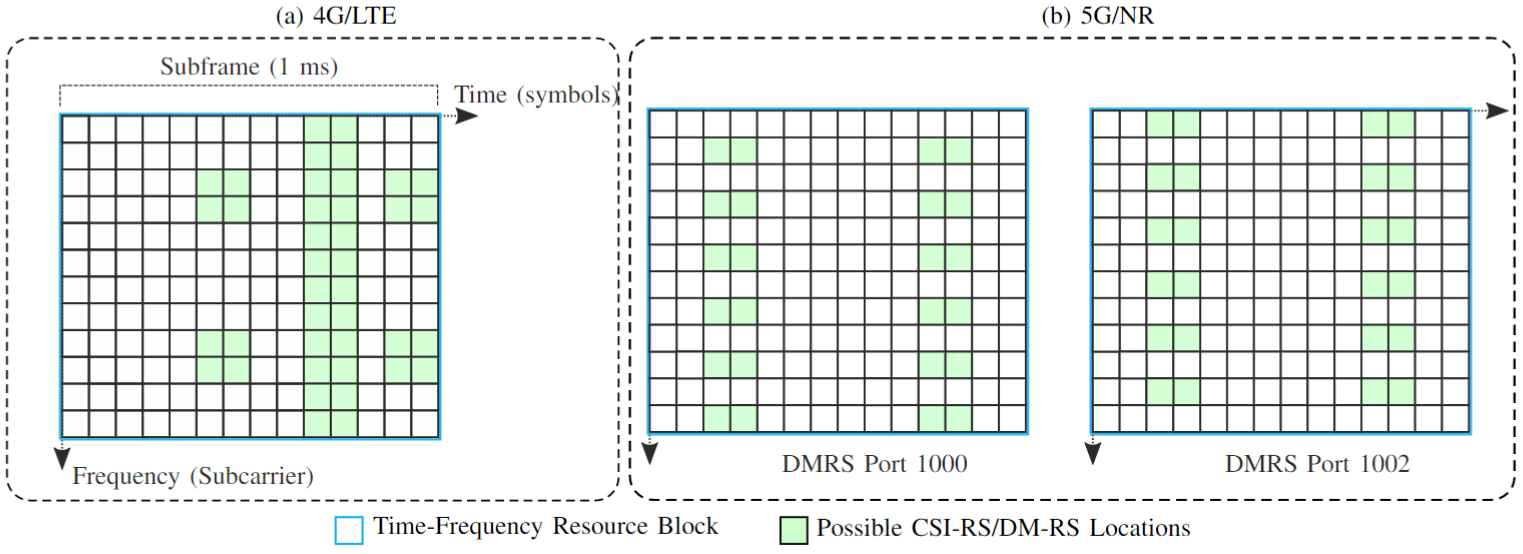
\includegraphics[width=\linewidth]{LTE_vs_5GNR_resource_grid.png}
    \caption{(a) LTE resource blocks with CSI-RS locations. (b) 5G NR resource blocks with DM-RS locations.}
    \label{fig:lte-vs-5g}
\end{figure}

While many using deep learning for CSI estimation do not address pilot estimation explicitly, a few works have incorporated pilot estimation into the CSI feedback problem. 

\section{Channel Model}
\label{sect:channel_model}

For all CSI tests, we mainly rely on the COST2100 MIMO channel model \cite{ref:liu2012cost2100}. We use two datasets with a single base station (gNB) and a single user equipment (UE) in the following scenarios:
\begin{enumerate}
	\item \textbf{Indoor} channels using a 5.3GHz downlink at
	0.001 m/s UE velocity, served by a
	gNB at center of a $20$m$\times 20$m coverage area.
	\item \textbf{Outdoor} channels using a 300MHz downlink at 0.9 m/s UE velocity served by a gNB at center 
	of a $400$m$\times 400$m coverage area.
\end{enumerate}
In both scenarios, we use the parameters listed in Table~\ref{tab:cost-params}.
\begin{table}[]
\centering
\caption{Parameters used for COST2100 simulations for both Indoor and Outdoor datasets.}
\label{tab:cost-params}
\begin{tabular}{c|c|l}
\toprule
\textbf{Symbol} & \textbf{Value} & \textbf{Description} \\ \midrule
$N_b$ 			& 32			 & Number of antennas at gNB  \\ \hline
$N_f$ 			& 1024			 & Number of subcarriers for OFDM link  \\ \hline
$R_d$ 			& 32			 & Number of delay elements kept after truncation  \\ \hline
$N$ 			& $10^6$		 & Total number of samples per dataset  \\ \hline
$T$ 			& 10		 	 & Number of timeslots  \\ \hline
$\delta$		& 40 ms			 & Feedback delay interval between consecutive CSI timeslots  \\ \bottomrule
\end{tabular}
\end{table}

\section{Classical CSI Estimation}
\label{sect:classic_estimation}

Works in compressive feedback for CSI estimation in MIMO networks can be placed in three broad categories. The first category includes works which use direct quantization of continuous CSI elements to discrete levels. The quantized CSI are encoded and fed back to the transmitter \cite{ref:makki2012hybrid,ref:shirani2009channel}. The second category includes works which use compressed sensing, a technique which applies a random measurement matrix at the transmitter and the receiver \cite{ref:rao2014distributed, ref:eltayeb2014compressive}. Compressed sensing assumes matrices to be encoded and fed back meet certain sparsity requirements, and compressed sensing algorithms require iterative solvers \cite{ref:do2008sparsity} for decoding, resulting in undesired latency.

The last category of work in compressive CSI feedback uses deep learning (DL), neural networks with numerous layers which are trained on large datasets using backpropagation. Before describing these works, we first describe a few pertinent concepts from deep learning.

\section{Deep Learning Background}
\label{sect:dl_overview}

This section provides a brief overview of relevant deep learning concepts employed in this work, including convolutional neural networks (CNNs), autoencoders, and unsupervised learning.

\textbf{Deep learning (DL)} is a subset of machine learning (ML), a broad class of algorithms which use data to ``fit'' models for prediction or classification tasks. The three predominant learning frameworks are supervised learning, unsupervised learning, and reinforcement learning. In the works proposed, we focus on \emph{unsupervised learning}, which seeks to find a compressed representation of the data without labels (see Chapter 14 of \cite{ref:Hastie2016Elements} for an overview).

\textbf{Convolutional Neural Networks}: A neural network is a machine learning algorithm with multiple \emph{layers} of parameterized linear functions followed nonlinear functions (typically referred to as `activation' functions). The parameters for these layers can be updated via a stochastic optimizer (e.g., \cite{ref:Kingma2014ADAM}), and given enough layers, such networks can achieve arbitrarily accurate functional approximation \cite{ref:Hecht1992TheoryBackprop}. In recent years, neural networks with convolutional layers have established state-of-the-art performance in computer vision tasks such as image classification \cite{ref:Sabour2017Dynamic} and segmentation \cite{ref:He2017Mask}.

\begin{figure}[!hbtp]
\centering
\def\svgwidth{0.8\columnwidth}
\input{images/autoencoder_schematic.pdf_tex}
\caption{Abstract schematic for an autoencoder operating on CSI matrices $\mathbf H$. The encoder learns a latent representation, $\mathbf Z$, while the decoder learns to reconstruct estimates $\hat{\mathbf H}$.}
\label{fig:autoencoder_schematic}
\end{figure}

A common architecture for deep unsupervised learning is the \emph{autoencoder} (see Fig.~\ref{fig:autoencoder_schematic} for a generic example). Trained end-to-end on input data, an autoencoder is comprised of an encoder and a decoder which jointly learn a compressed latent representation ($\mathbf Z$) and an estimate of the input ($\hat{\mathbf H}$). By choosing $\mathbf Z$ to have lower dimension than the input, the network is forced to learn a ``useful'' summary of the input data. The typical objective function for such a network is the mean squared error (MSE),
\begin{align*}
\underset{\theta_e, \theta_d}{\text{argmin}}\; \frac 1N \sum_{i=1}^N\Arrowvert \mathbf H_i - g(f(\mathbf H_i, \theta_e), \theta_d) \Arrowvert^2.
\end{align*}
We optimize network parameters $\vec \theta_e, \vec \theta_d$ by backpropagation and a stochastic optimization algorithm (e.g., stochastic gradient descent, ADAM).

\section{Objective and Contributions}

Successful efforts in DL for CSI estimation have typically utilized convolutional neural networks (CNNs) in an autoencoder structure \cite{ref:csinet}. Variations on the CNN-based autoencoder have investigated different network architectures \cite{ref:Lu2020CRNet}, variational training frameworks \cite{ref:Hussien2020PRVNet}, and denoising modules \cite{ref:Sun2020AnciNet}. These architectural changes are largely inspired by successful application of DL in image compression \cite{ref:szegedy2017inception,ref:balle2017end,ref:xie2012image}.

While they can continue to push the state-of-the-art in CSI reconstruction accuracy, architectural optimizations may ultimately follow the same trends of fields such as language modeling, where state-of-the-art performance requires prohibitively massive compute \cite{ref:brown2020language}. In this proposal, we take a different approach seek to improving compressive channel feedback by focusing on domain knowledge and physical insight.
% While the powerful functional approximation of deep CNNs has enabled state-of-the-art CSI reconstruction accuracy, they run the risk falling into the same trap as the image.

This qualifying exam proposal details our attempts to use domain knowledge to enhance the performance and the efficiency of neural networks for CSI estimation (for a visual summary, see Figure~\ref{fig:contrib}). Section~\ref{chap:sph_norm} details our work in power-based normalization, which leverages CSI sparsity. Section ~\ref{chap:markovnet} describes our work in differential encoding, which exploits temporal coherence of CSI. Section~\ref{chap:p2d} describes our work in pilot-based delay domain CSI estimation.

\begin{figure}[htb] \centering 
	{
	  \fontsize{4pt}{4pt}
	  \def\svgwidth{0.9\columnwidth}
	  % \input{images/cnns-venn-diagram-contrib.pdf_tex}
	}
	\caption{Venn diagram highlighting different aspects of domain knowledge in CNN-based CSI compressive feedback, relevant convolutional networks, and our contributions.}
	\label{fig:contrib}
\end{figure}